\documentclass[11pt,a4paper]{article}

\usepackage[utf8]{inputenc}
\usepackage[T1]{fontenc}
\usepackage[spanish,es-nodecimaldot]{babel}
\usepackage{lmodern}
\usepackage{amsmath,amssymb}
\usepackage{booktabs}
\usepackage{graphicx}
\usepackage{geometry}
\usepackage{microtype}
\usepackage{array}

\geometry{margin=2.5cm}
\setlength{\parindent}{0pt}
\setlength{\parskip}{0.55em}

\title{\textbf{Tarea 1: Resolución de EDO's y problemas de Control}}
\author{Tomás Serrano}
\date{14 de mayo de 2026}

\begin{document}

\begin{titlepage}
    \centering
    {\large Facultad de Ciencias Físicas y Matemáticas\par}
    {\large Universidad de Chile\par}
    \vspace{1.5cm}
    {\Large MA6914 Seminario Avanzado I\par}
    {\large Otoño 2026\par}
    \vfill
    {\LARGE\bfseries Tarea 1: Resolución de EDO's y problemas de Control\par}
    \vspace{1.5cm}
    {\large Tomás Serrano\par}
    \vfill
    \begin{tabular}{rl}
        Profesor: & Donato Vásquez \\
        Auxiliar: & Diego Olguín \\
        Fecha del enunciado: & 14 de mayo de 2026
    \end{tabular}
    \vfill
\end{titlepage}

\section{Introducción y alcance}

Este informe presenta la implementación y validación del integrador numérico de ecuaciones diferenciales ordinarias del Problema 1 y la infraestructura reutilizable para problemas de control óptimo tipo Bolza del Problema 2. El análisis se concentra en la convergencia y estabilidad observadas de los métodos de integración, y en la correspondencia entre la formulación matemática y la interfaz de control. Los Problemas 3 y 4 quedan fuera del alcance de este documento.

\section{Problema 1: integrador de EDO}

\subsection{Diseño e implementación}

Se considera el problema de valor inicial
\begin{equation}
    \dot{x}(t)=f\bigl(t,x(t),u(t)\bigr),
    \qquad x(t_0)=x_0,
    \qquad x(t)\in\mathbb{R}^n.
\end{equation}
La clase \texttt{EDOSolver} expone una interfaz única que recibe el campo, la condición inicial, el intervalo temporal, el paso y el método. Los cinco esquemas disponibles son Euler progresivo, Euler implícito, Heun, Crank--Nicolson y Runge--Kutta de orden cuatro (RK4). La clase \texttt{EDOSolution} almacena la grilla, los estados, el intervalo original y, opcionalmente, las etapas intermedias.

Los métodos explícitos evalúan directamente las pendientes requeridas por cada esquema. Euler implícito y Crank--Nicolson construyen, en cada paso, el residual no lineal correspondiente y lo resuelven mediante \texttt{scipy.optimize.fsolve}. La misma estructura admite dimensión de estado arbitraria, pasos efectivos ajustados a los extremos del intervalo y control opcional.

\subsection{Metodología de validación}

La verificación de orden usa el problema escalar $\dot{x}=-x$, cuya solución exacta es $e^{-t}$, y compara el cociente de errores al reducir el paso a la mitad. Las pruebas comprueban los órdenes esperados para Euler progresivo, Heun, Crank--Nicolson y RK4. Para los sistemas sin solución cerrada utilizada en los experimentos, el error se define por
\begin{equation}
    E_{\infty}=\max_{k,i}\left|x_{k,i}-x^{\mathrm{ref}}_i(t_k)\right|,
\end{equation}
donde la referencia se interpola cúbicamente sobre la grilla de la aproximación. Por tanto, este valor mide discrepancia respecto de una \emph{referencia numérica}; no es un error frente a una solución exacta y hereda la discretización e interpolación de dicha referencia.

\subsection{Sistema de Lotka--Volterra}

Se estudió
\begin{equation}
    \dot{x}=\alpha x-\beta xy,
    \qquad
    \dot{y}=\delta xy-\gamma y,
\end{equation}
con los parámetros oficiales $\alpha=1.1$, $\beta=0.4$, $\delta=0.1$, $\gamma=0.4$, condición inicial $(x(0),y(0))=(10,5)$ e intervalo $[0,15]$. La referencia numérica se calculó con Crank--Nicolson y $h=10^{-4}$.

\begin{figure}[htbp]
    \centering
    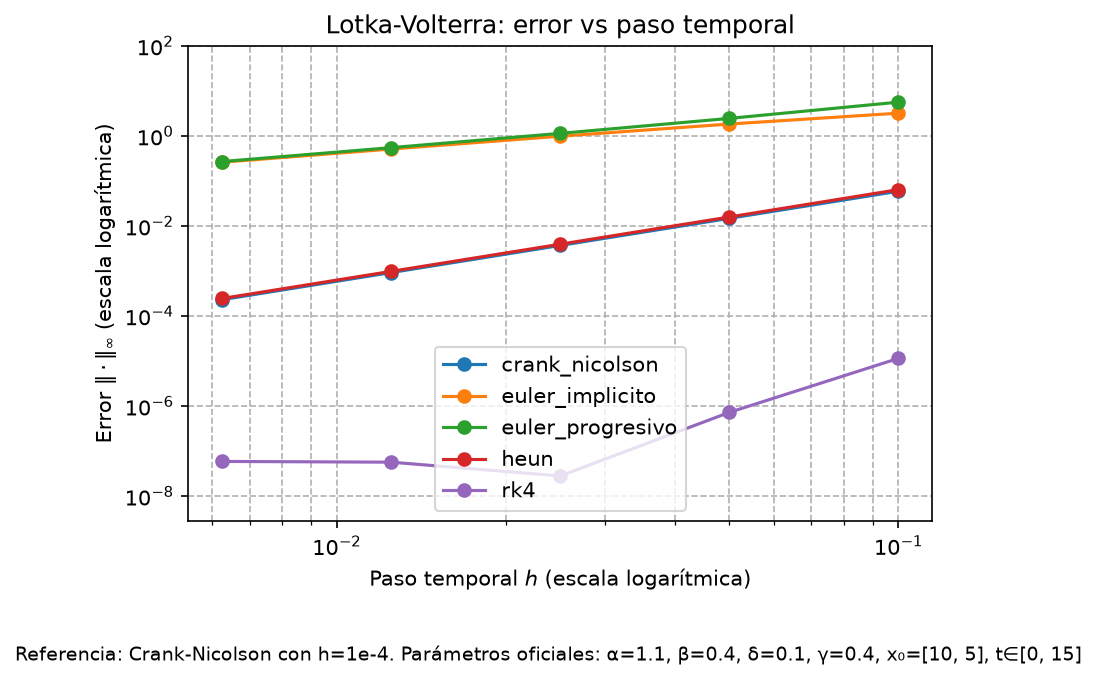
\includegraphics[width=0.82\textwidth]{assets/generated/problema1/lotka_volterra_error_vs_h.png}
    \caption{Error en norma infinito respecto de la referencia numérica Crank--Nicolson con $h=10^{-4}$. Se emplean los parámetros oficiales de Lotka--Volterra y pasos entre $0.1$ y $0.00625$.}
    \label{fig:lotka-error}
\end{figure}

La Figura~\ref{fig:lotka-error} muestra que el error disminuye al refinar la grilla. Euler progresivo e implícito presentan la reducción más lenta; Heun y Crank--Nicolson muestran un comportamiento de segundo orden; RK4 alcanza discrepancias considerablemente menores en los pasos ensayados, hasta aproximarse al límite impuesto por la referencia numérica.

\begin{figure}[htbp]
    \centering
    \begin{minipage}[t]{0.49\textwidth}
        \centering
        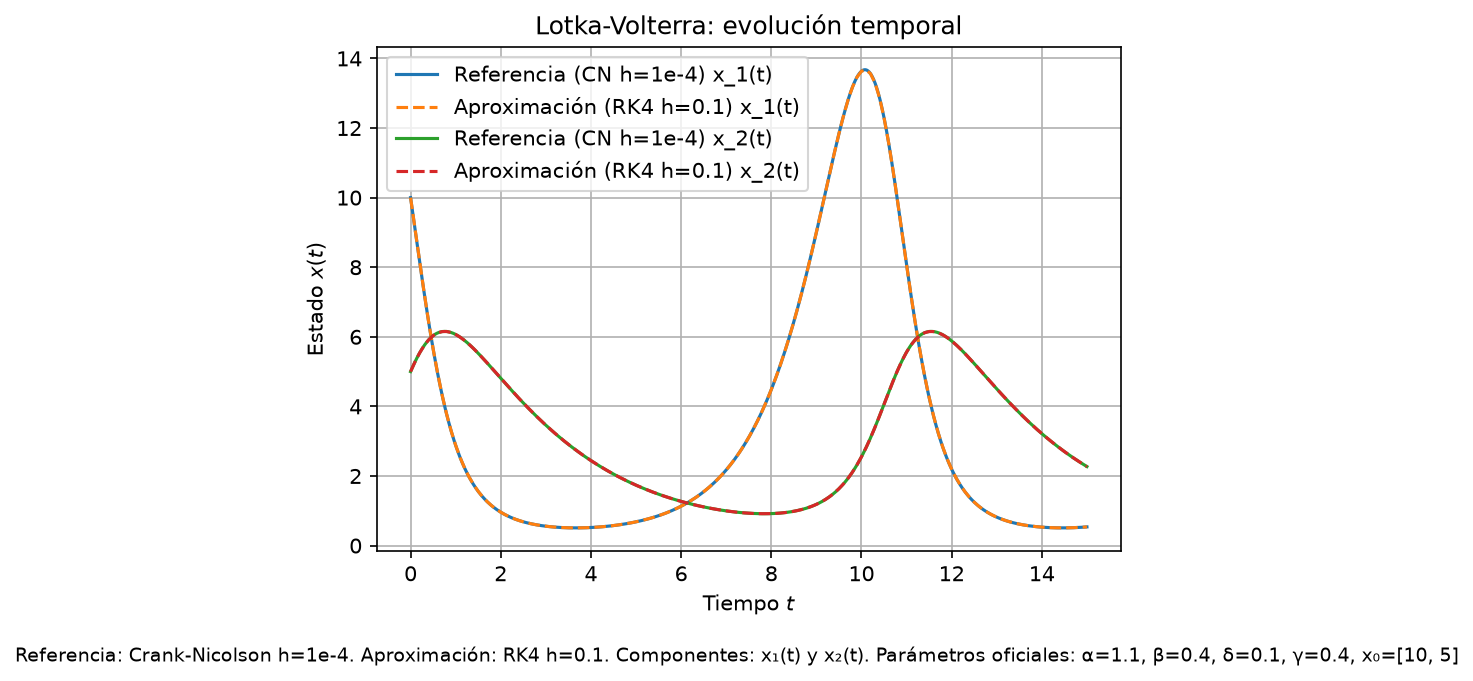
\includegraphics[width=\linewidth]{assets/generated/problema1/lotka_volterra_series_temporales.png}
        \small (a) Evolución temporal.
    \end{minipage}
    \hfill
    \begin{minipage}[t]{0.49\textwidth}
        \centering
        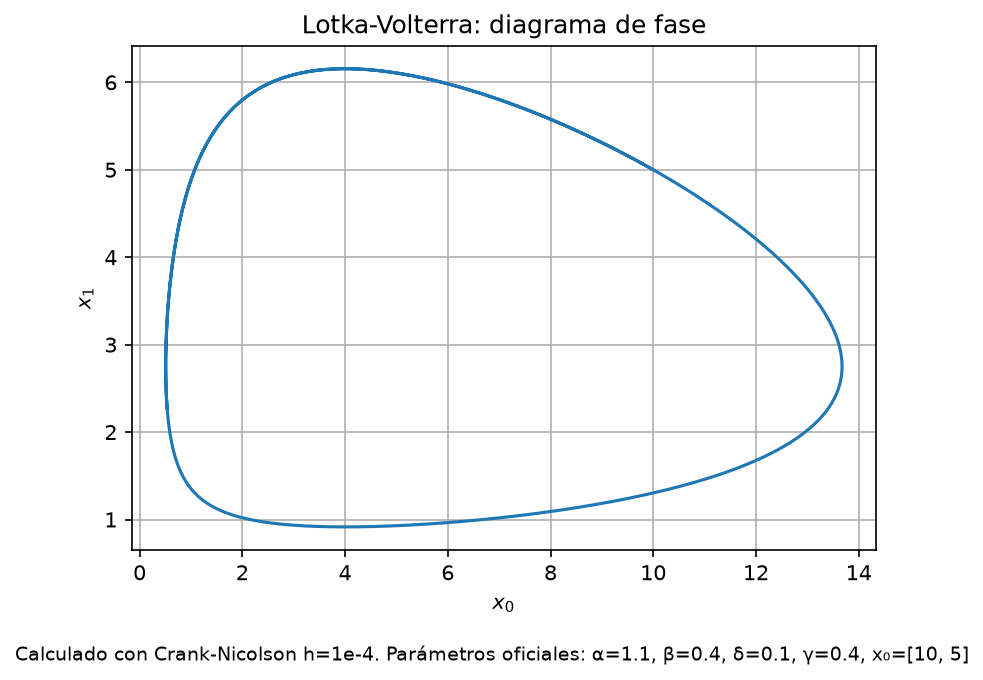
\includegraphics[width=\linewidth]{assets/generated/problema1/lotka_volterra_diagrama_fase.png}
        \small (b) Diagrama de fase de la referencia numérica.
    \end{minipage}
    \caption{Lotka--Volterra con $\alpha=1.1$, $\beta=0.4$, $\delta=0.1$, $\gamma=0.4$ y $(x(0),y(0))=(10,5)$. En (a), RK4 con $h=0.1$ se compara con la referencia numérica Crank--Nicolson con $h=10^{-4}$; en (b) se muestra la órbita calculada con esa referencia.}
    \label{fig:lotka-trayectorias}
\end{figure}

La superposición de las series temporales en la Figura~\ref{fig:lotka-trayectorias}(a) indica que RK4 con $h=0.1$ reproduce visualmente la referencia durante el intervalo estudiado. El diagrama de fase presenta la órbita cerrada característica de la interacción presa--depredador; esta figura también es numérica y no constituye una solución analítica.

\subsection{Oscilador de Van der Pol}

La ecuación
\begin{equation}
    \ddot{x}-\mu(1-x^2)\dot{x}+x=0
\end{equation}
se escribió como un sistema de primer orden con estado $(x,\dot{x})$ y condición inicial $(2,0)$. Se realizaron dos estudios claramente diferenciados. El caso $\mu=0.1$ es \emph{complementario}: permite comprobar el comportamiento de los métodos en un régimen suave, pero no sustituye el caso rígido solicitado. El estudio principal usa $\mu=1000$, $t\in[0,10]$ y una referencia numérica Crank--Nicolson con $h=10^{-5}$.

\begingroup
\small
\let\captiongenerada\caption
\renewcommand{\caption}[1]{\captiongenerada{Comparación entre tiempo observado y precisión para Van der Pol con $\mu=1000$.}}
\footnotesize\small
\let\detokenizeoriginal\detokenize
\def\detokenize#1{El tiempo medido proviene de una sola corrida; no constituye una referencia estable.}
\let\endtableoriginal\endtable
\renewcommand{\endtable}{\let\detokenize\detokenizeoriginal\endtableoriginal}
\begin{table}[htbp]
\centering
\caption{Van der Pol mu=1000: time-versus-precision comparison}
\label{tab:van-der-pol-mu-1000}
\begin{tabular}{lllll}
\hline
metodo & h & estado & error\_inf & tiempo\_s \\
\hline
euler\_progresivo & 1.00000000e-02 & no\_finito & No finito (NaN) & 3.34288480e-02 \\
euler\_progresivo & 5.00000000e-03 & no\_finito & No finito (NaN) & 3.84112240e-02 \\
euler\_progresivo & 2.50000000e-03 & no\_finito & No finito (NaN) & 9.68721780e-02 \\
euler\_progresivo & 1.25000000e-03 & no\_finito & No finito (NaN) & 9.42283600e-02 \\
heun & 1.00000000e-02 & no\_finito & No finito (NaN) & 6.80172790e-02 \\
heun & 5.00000000e-03 & no\_finito & No finito (NaN) & 7.42099870e-02 \\
heun & 2.50000000e-03 & no\_finito & No finito (NaN) & 1.52550528e-01 \\
heun & 1.25000000e-03 & no\_finito & No finito (NaN) & 3.27262294e-01 \\
rk4 & 1.00000000e-02 & no\_finito & No finito (NaN) & 1.52362152e-01 \\
rk4 & 5.00000000e-03 & no\_finito & No finito (NaN) & 2.34052986e-01 \\
rk4 & 2.50000000e-03 & no\_finito & No finito (NaN) & 3.07506686e-01 \\
rk4 & 1.25000000e-03 & no\_finito & No finito (NaN) & 7.98331750e-01 \\
euler\_implicito & 1.00000000e-01 & finito & 2.21503276e-06 & 3.31880800e-02 \\
euler\_implicito & 5.00000000e-02 & finito & 4.41520198e-06 & 6.99302070e-02 \\
euler\_implicito & 2.50000000e-02 & finito & 8.77211475e-06 & 1.18563412e-01 \\
euler\_implicito & 1.25000000e-02 & finito & 1.73161903e-05 & 2.14311916e-01 \\
euler\_implicito & 6.25000000e-03 & finito & 3.37554201e-05 & 7.74543779e-01 \\
crank\_nicolson & 1.00000000e-01 & finito & 6.57894115e-04 & 5.04521160e-02 \\
crank\_nicolson & 5.00000000e-02 & finito & 6.49150668e-04 & 4.08218650e-02 \\
crank\_nicolson & 2.50000000e-02 & finito & 6.32047730e-04 & 1.27532441e-01 \\
crank\_nicolson & 1.25000000e-02 & finito & 5.99161908e-04 & 2.29861283e-01 \\
crank\_nicolson & 6.25000000e-03 & finito & 5.38154879e-04 & 7.36123080e-01 \\
euler\_progresivo & 1.00000000e-05 & finito & 3.70718285e-06 & 2.19316907e+01 \\
euler\_progresivo & 5.00000000e-06 & finito & 1.83256233e-06 & 5.43357862e+01 \\
rk4 & 1.00000000e-05 & finito & 1.83965465e-08 & 1.55459429e+02 \\
rk4 & 5.00000000e-06 & finito & 1.83961552e-08 & 1.73173949e+02 \\
\hline
\end{tabular}
\par\smallskip
\footnotesize\detokenize{tiempo_s is one observed execution, not a stable benchmark.}
\end{table}

\endgroup

La tabla contiene 26 combinaciones: 14 produjeron estados y errores finitos, mientras que 12 produjeron valores no finitos. Estas 12 filas corresponden a Euler progresivo, Heun y RK4 con $h\in\{10^{-2},5\times10^{-3},2.5\times10^{-3},1.25\times10^{-3}\}$. El patrón es evidencia de inestabilidad numérica de los métodos explícitos bajo los pasos ensayados, no una demostración universal de divergencia.

En contraste, Euler implícito y Crank--Nicolson conservaron resultados finitos para pasos entre $0.1$ y $0.00625$. Euler progresivo y RK4 también produjeron resultados finitos al reducir el paso a $10^{-5}$ y $5\times10^{-6}$, con un costo temporal observado mucho mayor. Esto respalda la restricción de paso de los métodos explícitos en el régimen rígido y la mayor robustez de los implícitos con pasos más grandes.

La comparación cuantitativa exige dos cautelas. Primero, cada valor de \texttt{tiempo\_s} proviene de una sola ejecución y no debe interpretarse como un benchmark repetido. Segundo, los errores se calculan respecto de Crank--Nicolson con $h=10^{-5}$; por ello describen acuerdo con esa referencia y no precisión absoluta. Esta limitación también puede explicar tendencias no monótonas al refinar métodos implícitos cuando la diferencia alcanza la escala del error de referencia.

\section{Problema 2: clase reutilizable de control Bolza}

\subsection{Formulación matemática}

La clase \texttt{ControlProblem} representa el problema
\begin{equation}
    \min_{u}\;J[u]
    =\Phi\bigl(x(T)\bigr)
    +\int_{t_0}^{T}L\bigl(t,x(t),u(t)\bigr)\,dt,
\end{equation}
sujeto a
\begin{equation}
    \dot{x}(t)=f\bigl(t,x(t),u(t)\bigr),
    \qquad x(t_0)=x_0,
    \qquad u(t)\in U.
\end{equation}
El horizonte se entrega explícitamente como \texttt{t\_span}=$(t_0,T)$. El conjunto admisible puede ser irrestricto, $U=\mathbb{R}^m$, o una caja $U=[u_{\min},u_{\max}]$, cuya proyección por componentes se implementa mediante recorte a los límites.

Con el Hamiltoniano
\begin{equation}
    H(t,x,p,u)=L(t,x,u)+p^{\mathsf T}f(t,x,u),
\end{equation}
la dinámica adjunta y la condición terminal para estado final libre son
\begin{equation}
    \dot{p}(t)=-\frac{\partial H}{\partial x}
    =-\left(\frac{\partial L}{\partial x}
    +\left(\frac{\partial f}{\partial x}\right)^{\mathsf T}p\right),
    \qquad
    p(T)=\nabla\Phi\bigl(x(T)\bigr).
\end{equation}
La minimización puntual queda definida por
\begin{equation}
    u^{\star}(t)\in\operatorname*{arg\,min}_{u\in U}H(t,x(t),p(t),u).
\end{equation}
En dimensión escalar se emplea minimización unidimensional; para controles vectoriales se utiliza minimización con cotas. Cuando $U$ es una caja, el resultado respeta sus límites, de manera consistente con la proyección puntual sobre el conjunto admisible.

\subsection{Decisiones de implementación y verificación}

La infraestructura exige las cinco derivadas analíticas $\partial f/\partial x$, $\partial f/\partial u$, $\partial L/\partial x$, $\partial L/\partial u$ y $\nabla\Phi$; no se introduce una aproximación silenciosa por diferencias finitas. La evaluación de $J$ exige además un paso $h$ explícito, integra la trayectoria con el método seleccionado y aplica cuadratura trapezoidal al costo de operación.

\begin{table}[htbp]
    \centering
    \caption{Correspondencia entre requisitos del Problema 2 y verificaciones de la implementación.}
    \label{tab:control-problem}
    \small
    \begin{tabular}{>{\raggedright\arraybackslash}p{0.28\textwidth} >{\raggedright\arraybackslash}p{0.62\textwidth}}
        \toprule
        Componente & Verificación disponible \\
        \midrule
        Constructor reutilizable & Valida \texttt{t\_span}, dimensión del control, estado inicial, dimensión de la dinámica y presencia de las cinco derivadas analíticas. \\
        Conjunto admisible & Comprueba identidad con copia para $\mathbb{R}^m$, recorte por componentes para cajas y validación de límites. \\
        Hamiltoniano y adjunto & Contrasta $H=L+p^{\mathsf T}f$, la dimensión de $-\partial H/\partial x$ y la transversalidad $p(T)=\nabla\Phi(x(T))$. \\
        Evaluación de costo & Exige $h$, acepta controles como función o arreglo, verifica su equivalencia y contrasta la cuadratura con un caso escalar conocido. \\
        Control puntual & Verifica la minimización irrestricta escalar y el respeto de los límites en un caso con caja. \\
        \bottomrule
    \end{tabular}
\end{table}

El Problema 2 define infraestructura general y no solicita por sí solo un caso numérico independiente. Por ello, la Tabla~\ref{tab:control-problem} resume propiedades de interfaz y pruebas funcionales sin atribuir optimalidad global ni resultados numéricos no demostrados.

\section{Conclusiones}

La interfaz unificada permite aplicar cinco esquemas a sistemas vectoriales y conservar una representación común de sus soluciones. En Lotka--Volterra, el refinamiento reduce la discrepancia respecto de la referencia numérica y RK4 reproduce las trayectorias de referencia con alta concordancia visual para el paso mostrado. En Van der Pol con $\mu=1000$, los resultados observados evidencian que los métodos explícitos requieren pasos mucho menores para evitar valores no finitos, mientras que Euler implícito y Crank--Nicolson mantienen resultados finitos con pasos mayores; las conclusiones de precisión quedan condicionadas por la referencia Crank--Nicolson con $h=10^{-5}$.

La formulación del Problema 2 encapsula dinámica, costos, derivadas, horizonte y restricciones en un objeto reutilizable. La evaluación consistente del costo, el sistema adjunto, la transversalidad y la minimización puntual establecen la base para los algoritmos posteriores. Los Problemas 3 y 4 permanecen pendientes y no se analizan en este informe.

\end{document}
